\section{Architettura di Dettaglio - Frontend}

Questa sezione descrive nel dettaglio l'architettura dei moduli del frontend. Per mantenere la coerenza formale con il backend e fornire un'analisi rigorosa seppur nel paradigma Component-Based, i costrutti fondamentali come Service, Context Provider e Hook Custom vengono esplorati analiticamente come singoli moduli ("classi").

\subsection{Servizi di Accesso Dati (Service Facade)}

\paragraph{cartService}
\vspace{\baselineskip}\noindent\textbf{Descrizione della classe:} modulo Singleton che funge da Facade per la comunicazione asincrona col backend in materia di carrello. Abstrae i dettagli della libreria \texttt{apiClient} (HTTP fetch e proxying).

\vspace{\baselineskip}\noindent\textbf{Descrizione degli attributi:} il modulo non possiede attributi di stato interni, in quanto il dominio del carrello è demandato al \texttt{CartContext}.

\vspace{\baselineskip}\noindent\textbf{Descrizione dei metodi:}
\begin{itemize}
    \item \texttt{getCart(sessionId?)}: recupera il carrello attivo formattando il DTO in un array \texttt{CartItem[]}.
    \item \texttt{addItem(codArt, qta, extra?)}: aggiunge un nuovo articolo al carrello della sessione corrente.
    \item \texttt{removeItem(id, sessionId?)}: rimuove una riga ordine specifica.
    \item \texttt{updateQty(id, qta, source, sessionId?)}: aggiorna le quantità tenendo traccia dell'origine dell'evento (es. "customer" o "ai").
    \item \texttt{addByName(productName, qta, sessionId?)}: aggiunge elementi effettuando lookup testuale pilotato dal backend.
    \item \texttt{addByCode(codArt, qta, sessionId?)}: aggiunta precisa di elementi tramite \texttt{cod\_art}.
\end{itemize}

\begin{figure}[H]
    \centering
    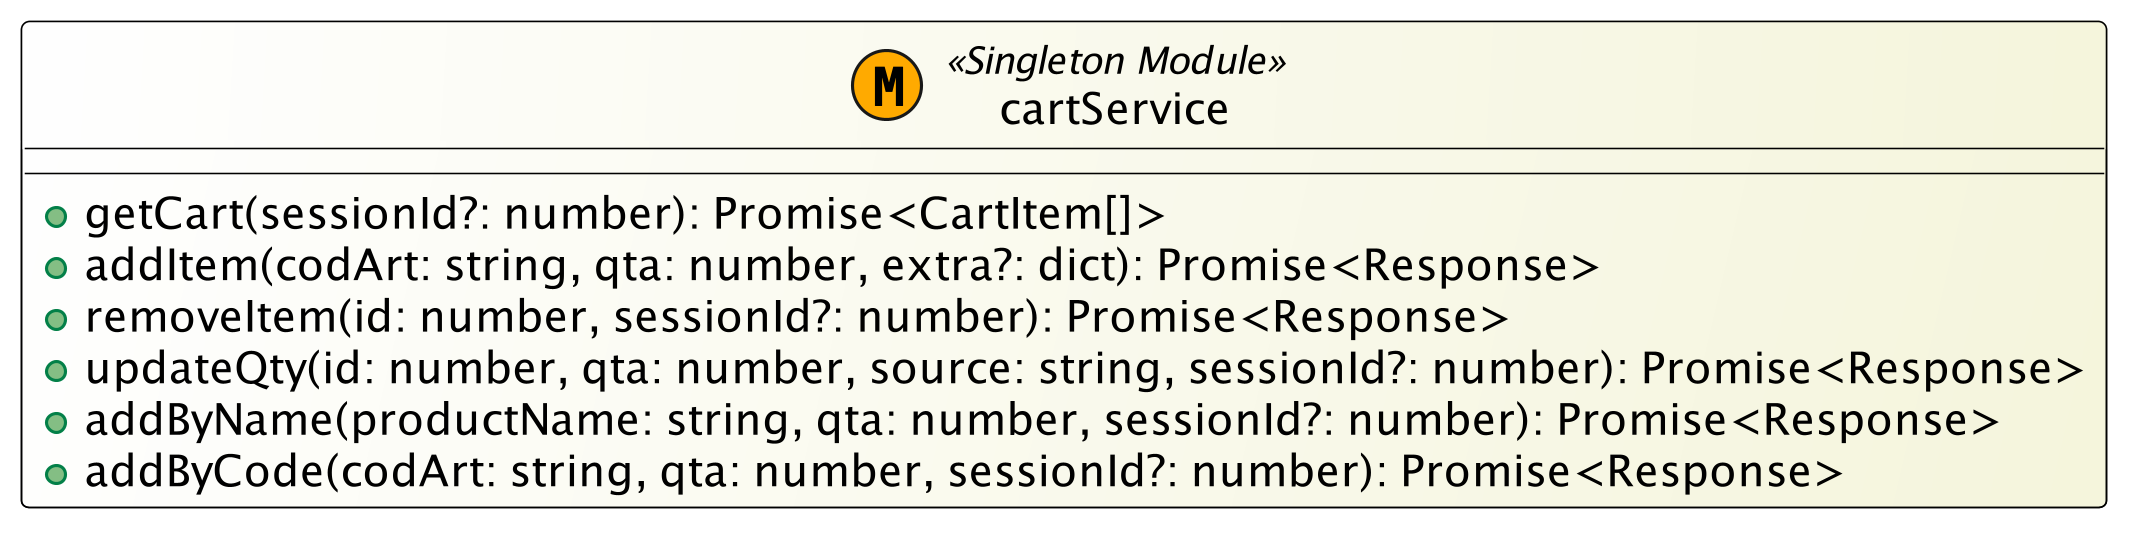
\includegraphics[width=0.62\textwidth]{componenti_specifiche_tecniche/assets/uml_frontend/01_cartService.png}
    \caption{UML del modulo \texttt{cartService}.}
\end{figure}


\paragraph{chatService}
\vspace{\baselineskip}\noindent\textbf{Descrizione della classe:} modulo per incapsulare la complessa interazione utente-assistente e delegarla agli end-point API deputati all'AI.

\vspace{\baselineskip}\noindent\textbf{Descrizione degli attributi:} puramente stateless.

\vspace{\baselineskip}\noindent\textbf{Descrizione dei metodi:}
\begin{itemize}
    \item \texttt{sendMessage(...)}: invia stringhe all'LLM e processa la risposta applicativa composita (incluse \texttt{ChatApiResponse} con intenzioni e modifiche carrello).
    \item \texttt{getMessages(sessionId)}: ripristina la persistenza dei messaggi in RAM recuperandola nel formato di dominio \texttt{Message[]}.
    \item \texttt{saveMessage(sessionId, sender, content)}: memorizza unilateralmente un messaggio offline.
    \item \texttt{transcribe(audioBlob)}: instrada il media blob verso Whisper (Backend API).
    \item \texttt{uploadImage(imageBlob, sessionId?)}: gestisce l'upload asincrono dell'immagini per analisi OCR.
\end{itemize}

\begin{figure}[H]
    \centering
    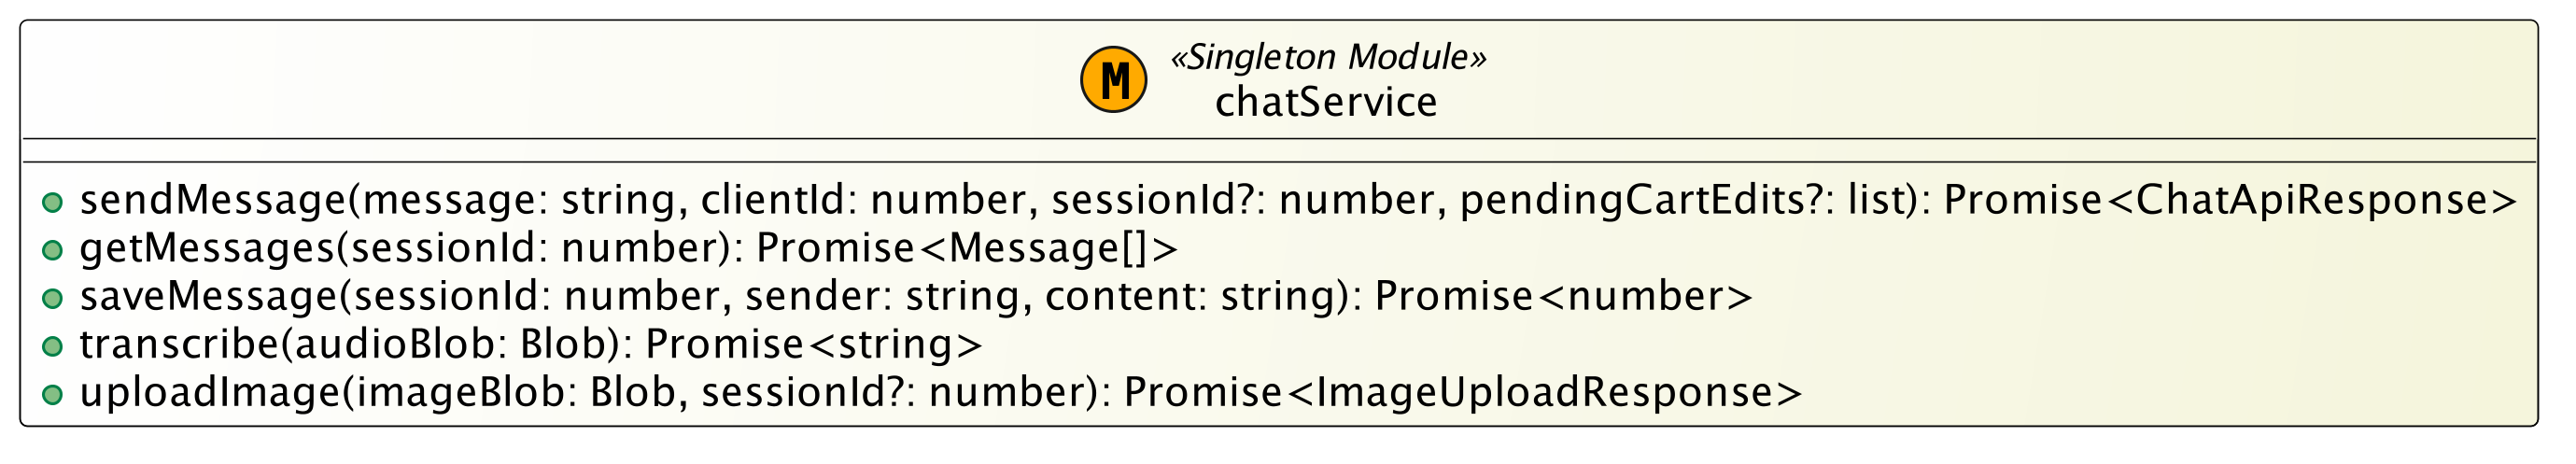
\includegraphics[width=0.62\textwidth]{componenti_specifiche_tecniche/assets/uml_frontend/02_chatService.png}
    \caption{UML del modulo \texttt{chatService}.}
\end{figure}


\paragraph{authService}
\vspace{\baselineskip}\noindent\textbf{Descrizione della classe:} gestore dell'identità. Offre metodi per la pre-autenticazione, la negoziazione del token JWT con cookie HTTPOnly e il recupero del ruolo operatore o cliente.

\vspace{\baselineskip}\noindent\textbf{Descrizione degli attributi:} non porta con sé stati locali del token (questo per via dell'utilizzo di cookie gestiti dal browser o dal server Next.js).

\vspace{\baselineskip}\noindent\textbf{Descrizione dei metodi:}
\begin{itemize}
    \item \texttt{login(email, password, codCli?)}: negozia le credentials per ricevere session cookies e path di reindirizzamento.
    \item \texttt{getProfile()}: ritorna un'interfaccia \texttt{UserProfile} tipizzata.
    \item \texttt{logout()}: invoca la distruzione di sessione back-end e locale.
    \item \texttt{changePassword(current, newPwd)}: routine protetta di aggiornamento credenziali.
    \item \texttt{getExportFolder()}: recupera l'albero di directory d'esportazione dall'istanza utente.
    \item \texttt{setExportFolder(path)}: applica le preferenze relative all'export degli ordini da file system.
\end{itemize}

\begin{figure}[H]
    \centering
    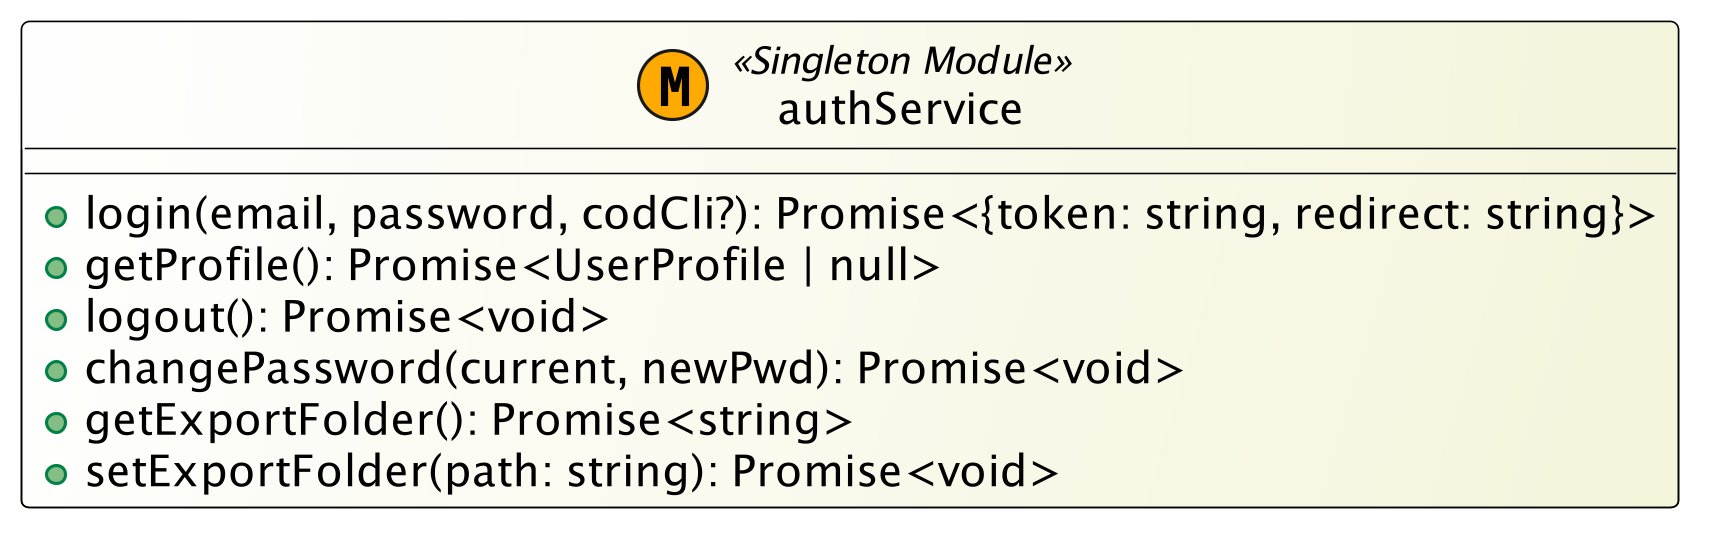
\includegraphics[width=0.62\textwidth]{componenti_specifiche_tecniche/assets/uml_frontend/03_authService.png}
    \caption{UML del modulo \texttt{authService}.}
\end{figure}

\paragraph{productService}
\vspace{\baselineskip}\noindent\textbf{Descrizione della classe:} modulo che gestisce l'interfacciamento con le logiche del backend per la navigazione del catalogo prodotti.
\vspace{\baselineskip}\noindent\textbf{Descrizione degli attributi:} stateless.
\vspace{\baselineskip}\noindent\textbf{Descrizione dei metodi:}
\begin{itemize}
    \item \texttt{search(query)}: riceve input parziali, codifica l'URL e interroga il db vector/keywords restituendo una \texttt{Promise<Product[]>}.
\end{itemize}

\begin{figure}[H]
    \centering
    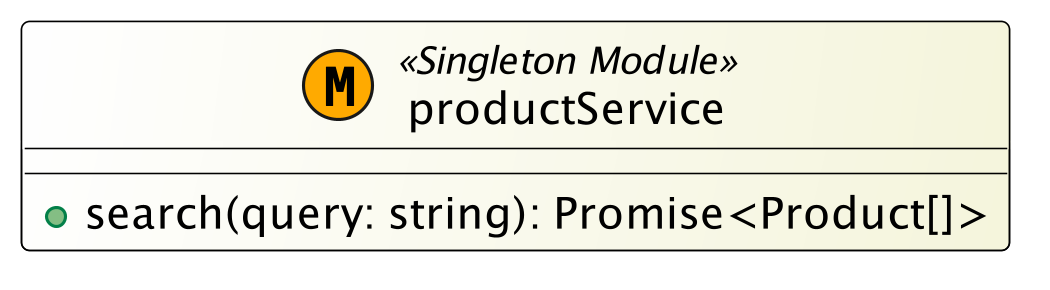
\includegraphics[width=0.62\textwidth]{componenti_specifiche_tecniche/assets/uml_frontend/09_productService.png}
    \caption{UML del modulo \texttt{productService}.}
\end{figure}


\paragraph{orderService}
\vspace{\baselineskip}\noindent\textbf{Descrizione della classe:} esegue la facade per tutte le view relative allo storico ordini (cliente) o alla dashboard panoramica (backoffice operatore).
\vspace{\baselineskip}\noindent\textbf{Descrizione degli attributi:} stateless.
\vspace{\baselineskip}\noindent\textbf{Descrizione dei metodi:}
\begin{itemize}
    \item \texttt{listAll(filters?)}: restituisce l'aggregato ordini globale.
    \item \texttt{list(codCli, page?, filters?)}: restituisce la pagina di ordini di uno specifico cliente.
    \item \texttt{detail(orderId)}: recupera interamente un \texttt{OrderDetail} inclusivo di righe carrello.
    \item \texttt{exportSelection(selectedIds)}: inoltra una richiesta massiva al server per l'export su disco.
    \item \texttt{downloadExported()}: avvia il download del buffer binario (Zip/Excel) precedentemente elaborato.
\end{itemize}

\begin{figure}[H]
    \centering
    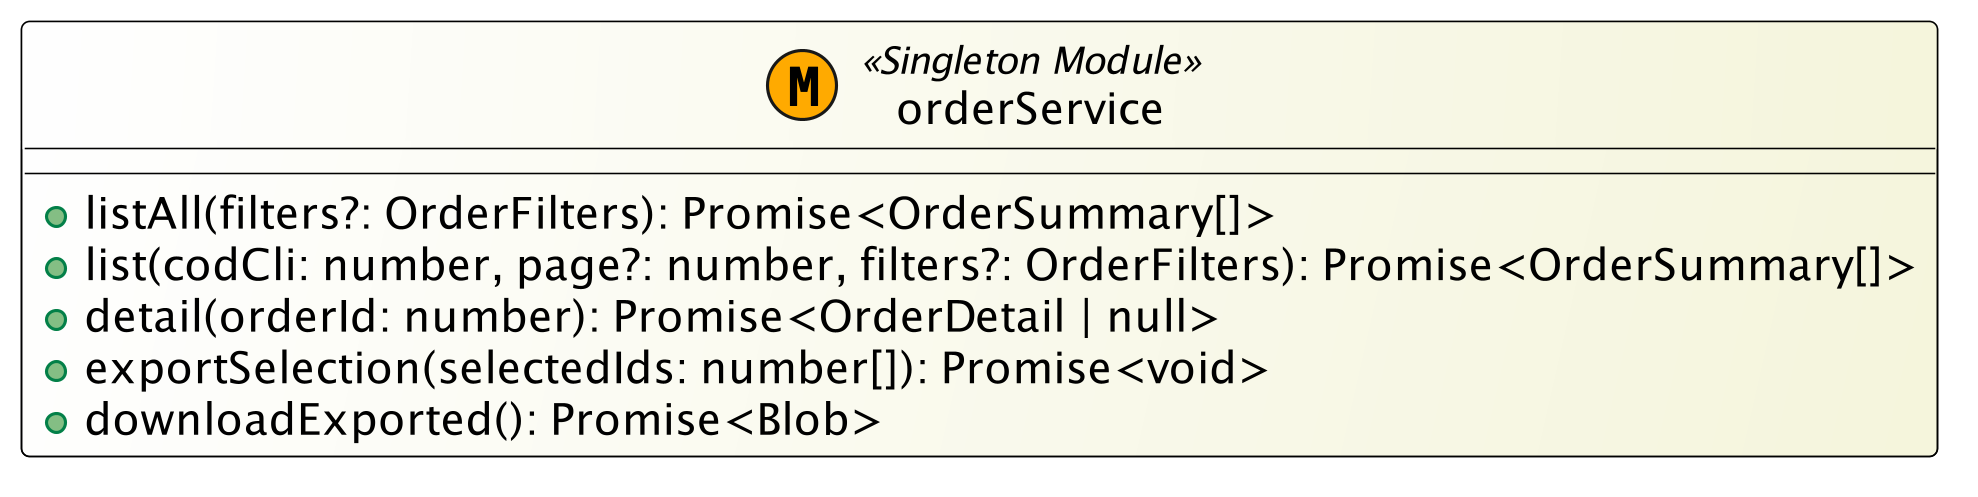
\includegraphics[width=0.62\textwidth]{componenti_specifiche_tecniche/assets/uml_frontend/07_orderService.png}
    \caption{UML del modulo \texttt{orderService}.}
\end{figure}


\paragraph{ticketService}
\vspace{\baselineskip}\noindent\textbf{Descrizione della classe:} facade utilizzata dagli operatori del Customer Care per la gestione delle casistiche delegate dal Bot.
\vspace{\baselineskip}\noindent\textbf{Descrizione degli attributi:} stateless.
\vspace{\baselineskip}\noindent\textbf{Descrizione dei metodi:}
\begin{itemize}
    \item \texttt{getOpenTickets()}: popola la tabella principale del backoffice con ticket inevasi.
    \item \texttt{getTicketDetail(ticketId)}: recupera i dati del singolo ticket e della chat utente annessa.
    \item \texttt{lockTicket(ticketId) / unlockTicket(ticketId)}: transazioni di locking competitivo per presa in carico esclusiva dell'operatore.
    \item \texttt{closeTicket(ticketId, recap)}: risolve il ticket inserendo un recap di chiusura.
    \item \texttt{sendMessage(ticketId, content)}: inietta un messaggio asincrono bypassando l'AI per comunicare con l'utente target.
    \item \texttt{getPlatformOverview()}: fornisce le metriche statistiche e l'array di andamento per la root della dashboard.
\end{itemize}

\begin{figure}[H]
    \centering
    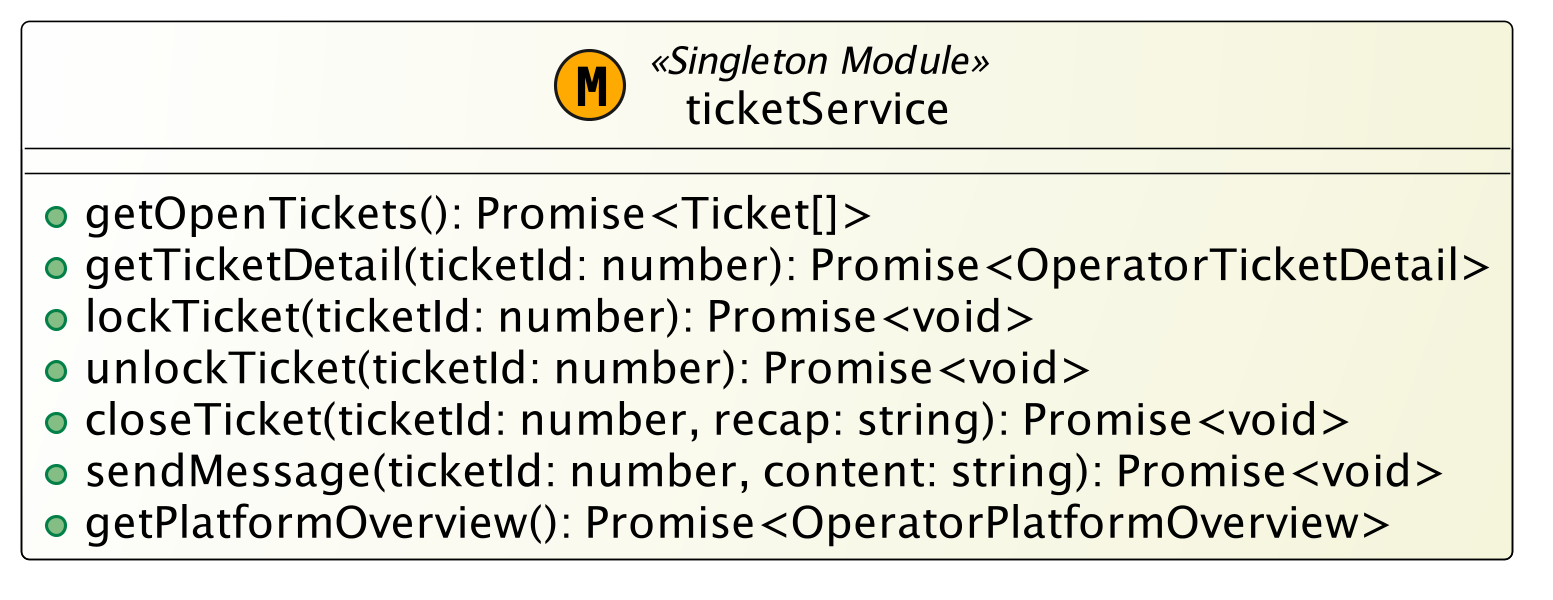
\includegraphics[width=0.62\textwidth]{componenti_specifiche_tecniche/assets/uml_frontend/08_ticketService.png}
    \caption{UML del modulo \texttt{ticketService}.}
\end{figure}


\paragraph{sessionService \textit{\& Altri (feedbackService, healthService, apiClient)}}
\vspace{\baselineskip}\noindent\textbf{Descrizione della classe:} raggruppamento di moduli minori per la diagnostica, metriche e la sessione esplicita. Da includere la libreria fondamentale \texttt{apiClient}.
\vspace{\baselineskip}\noindent\textbf{Descrizione degli attributi:} le utilities interne mantengono scope protetti sul modulo originario.
\vspace{\baselineskip}\noindent\textbf{Descrizione dei metodi:}
\begin{itemize}
    \item \texttt{sessionService.getActive()}: rintracciabilità dell'handshake primario.
    \item \texttt{sessionService.create()}: crea esplicitamente una sessione per uno specifico ID cliente in assenza di cookie.
    \item \texttt{feedbackService.submit(messageId, isPositive, reason?, comment?)}: inoltro del rating e feed di rinforzo sul modello.
    \item \texttt{healthService.check()}: pooling verso servizi esterni (status AI).
    \item \texttt{apiClient.apiFetch(path, init?)}: override globale per iniezione di cookie/CORS preflight.
    \item \texttt{apiClient.getApiErrorMessage(response, fallback)}: standardizza i payload JSON per l'estrazione granulare dell'errore (risoluzione 422 vs 500).
    \item \texttt{apiClient.buildApiUrl(path)}: prefissa consistentemente con lo snippet basePath.
    \item \texttt{apiClient.getApiBaseUrl()}: switcha gli use states ambientali (Dev locale proxata Next.js versus FastAPI puro).
\end{itemize}

\begin{figure}[H]
    \centering
    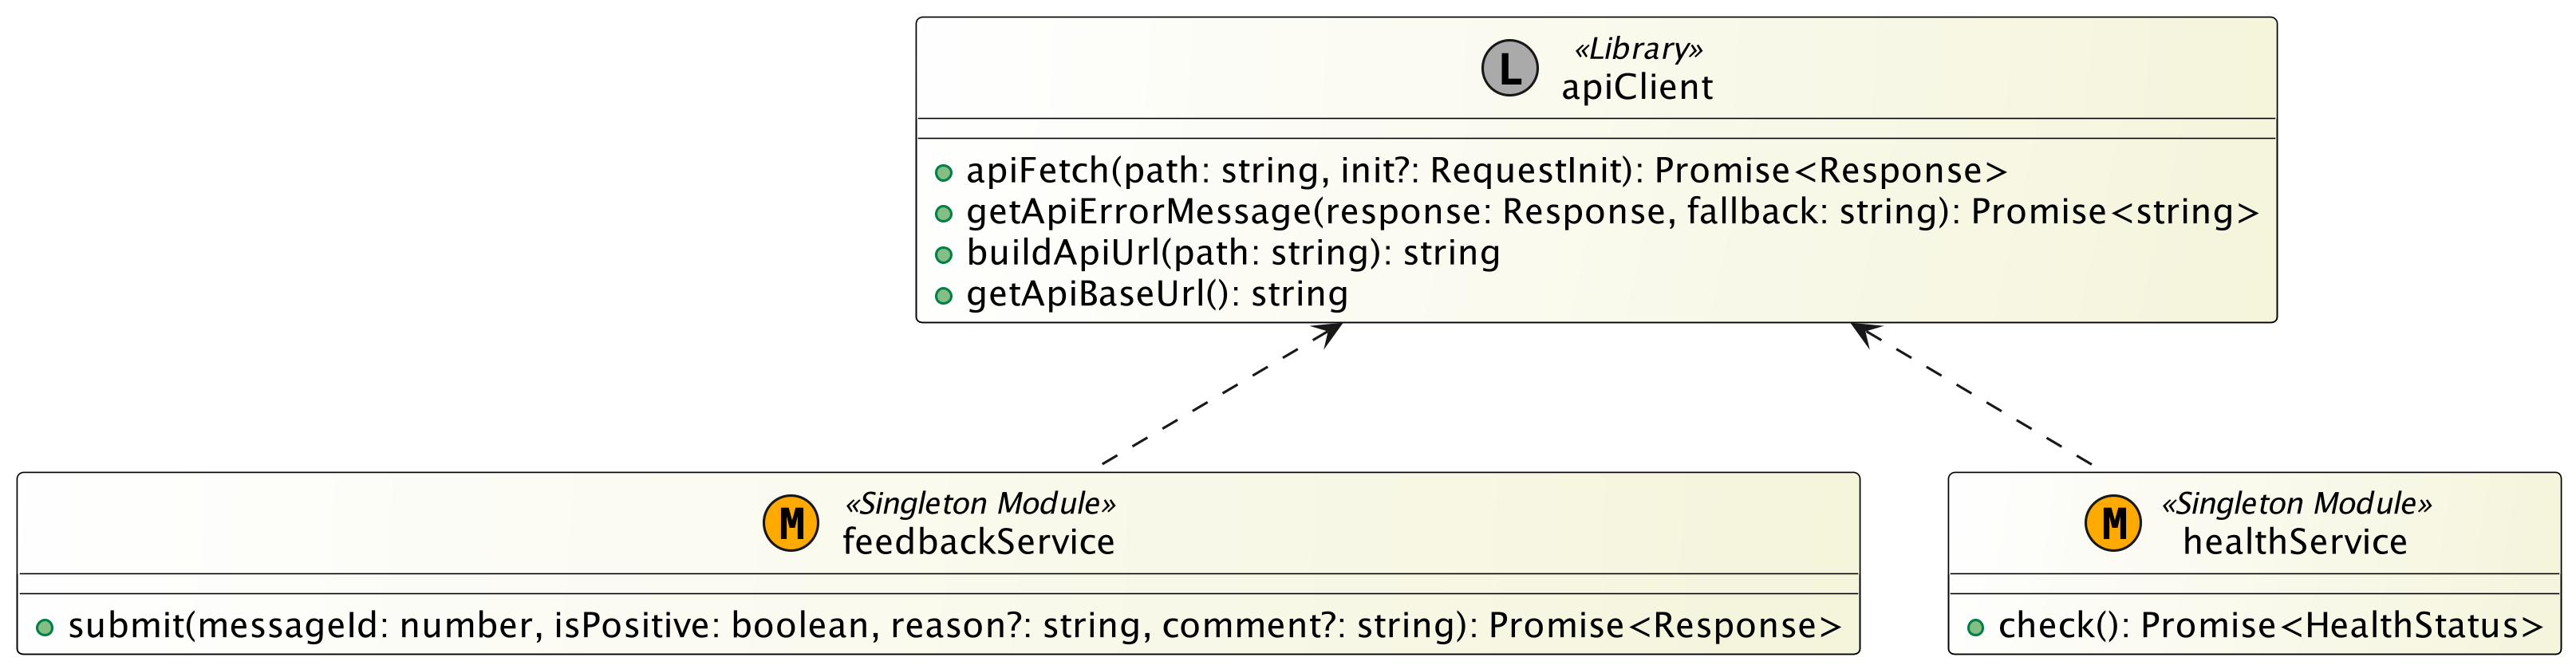
\includegraphics[width=0.90\textwidth]{componenti_specifiche_tecniche/assets/uml_frontend/11_otherServices.png}
    \caption{UML dei moduli minori e della libreria \texttt{apiClient}.}
\end{figure}


\subsection{Contesti e Stato Applicativo (React Contexts)}

\paragraph{SessionContext}
\vspace{\baselineskip}\noindent\textbf{Descrizione della classe:} Provider architetturale React che isola la cronologia logica di interazione (Bot e Umano) per l'utente, governando lo stato dinamico e disaccoppiandolo dai componenti visuali. Il two-way binding dello stato è risolto implicitamente e automaticamente dai re-render del Virtual DOM di React al mutare del Context (implementazione concreta dell'Observer pattern applicata all'UI).

\vspace{\baselineskip}\noindent\textbf{Descrizione degli attributi:}
\begin{itemize}
    \item \texttt{sessionId}: identificativo univoco della transazione corrente associata a un cliente.
    \item \texttt{chatMessages}: array di storicizzazione in RAM di dominio \texttt{Message[]}.
    \item \texttt{showNewSessionModal}: flag di overlay per interrompere / generare sessioni.
\end{itemize}

\vspace{\baselineskip}\noindent\textbf{Descrizione dei metodi:}
\begin{itemize}
    \item \texttt{initSession()}: richiede l'inizializzazione server di una track.
    \item \texttt{handleNewSession() / confirmNewSession()}: orchestra l'alert state.
    \item \texttt{cancelNewSession()}: annulla la creazione di una nuova sessione dismissando il modale protettivo.
    \item \texttt{setChatMessages(messages)}: dispatcher esposto per l'aggiornamento dei widget sottoscritti nella gerarchia React.
\end{itemize}

\begin{figure}[H]
    \centering
    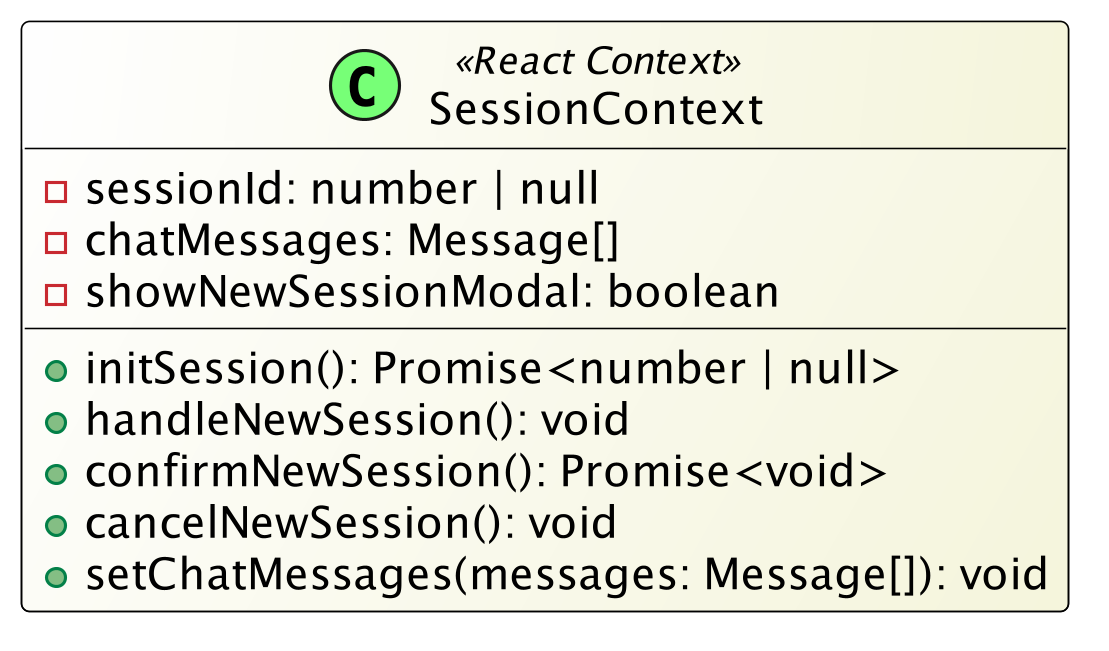
\includegraphics[width=0.62\textwidth]{componenti_specifiche_tecniche/assets/uml_frontend/04_SessionContext.png}
    \caption{UML del Provider \texttt{SessionContext}.}
\end{figure}


\paragraph{CartContext}
\vspace{\baselineskip}\noindent\textbf{Descrizione della classe:} React Provider core del sistema, accentra e consolida le logiche di aggiornamento \textit{Optimistic UI}.

\vspace{\baselineskip}\noindent\textbf{Descrizione degli attributi:}
\begin{itemize}
    \item \texttt{cart}: iterabile di articoli correnti (\texttt{CartItem[]}).
    \item \texttt{pendingUpdates}: Ref di memoria interno che mappa ID prodotto su specifici Timer di \textit{Debounce map}, per rinviare sincronizzazioni a basso delta temporale dirette al backend.
\end{itemize}

\vspace{\baselineskip}\noindent\textbf{Descrizione dei metodi:}
\begin{itemize}
    \item \texttt{refreshCart()}: innesca un overlay pulito scaricando la source of truth remota.
    \item \texttt{addItem(codArt, qta, extra?)}: gestore accodamento, triggera implicitamente il Refresh state.
    \item \texttt{removeItem(id)}: annulla l'oggetto da visualizzare.
    \item \texttt{updateQty(id, qta, source?)}: gestisce l'incremento di UI ottimistica, sopprimendo e ritardando l'effettiva request a 600ms per salvaguardare le performance.
    \item \texttt{clearCart()}: ripristina la referenza globale svuotando passivamente gli array di visualizzazione.
    \item \texttt{hasPendingUpdates()}: esegue una size introspection sul map del timer (es. per bloccare la redirect di UI quando ci sono flussi non confermati).
\end{itemize}

\begin{figure}[H]
    \centering
    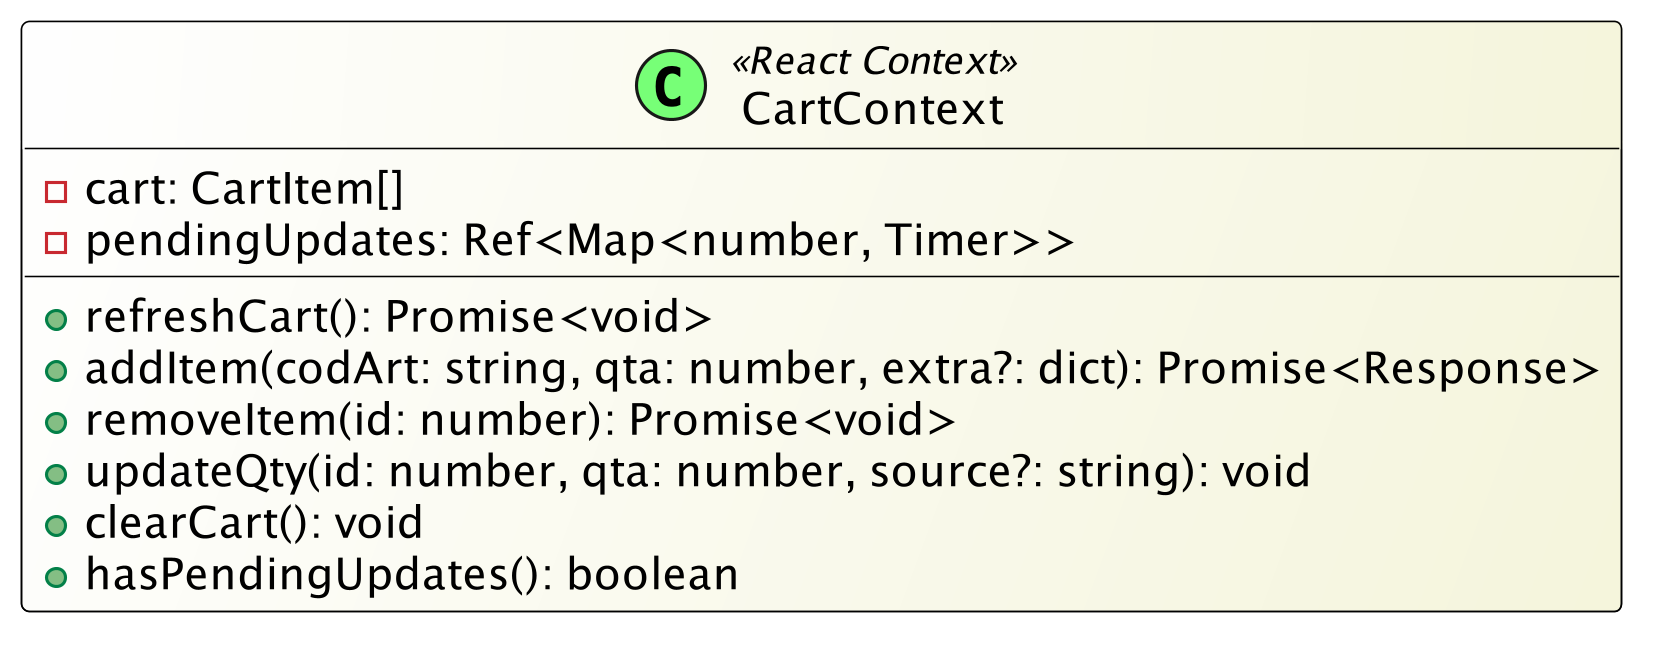
\includegraphics[width=0.62\textwidth]{componenti_specifiche_tecniche/assets/uml_frontend/05_CartContext.png}
    \caption{UML del Provider \texttt{CartContext}.}
\end{figure}


\subsection{Flussi Asincroni (Custom Hooks)}

\paragraph{useSSE}
\vspace{\baselineskip}\noindent\textbf{Descrizione della classe:} Custom Hook isolato il cui scopo è gestire la negoziazione e la latenza dei \texttt{Server-Sent Events} con policy reattive verso l'interfaccia.

\vspace{\baselineskip}\noindent\textbf{Descrizione degli attributi:}
\begin{itemize}
    \item \texttt{connected}: booleano derivato in tempo reale.
    \item \texttt{reconnectAttempts}: conteggio incrementale dei fallimenti via backoff esponenziale.
    \item \texttt{esRef}: EventSource raw instance allocata non-reattivamente.
\end{itemize}

\vspace{\baselineskip}\noindent\textbf{Descrizione dei metodi:}
\begin{itemize}
    \item \texttt{connect()}: routine auto-rigenerativa preposta per il bootstrap o retrail di una stream socket.
    \item \texttt{fetchSSEToken()}: interfaccia il proxy bridge per ricavare credenziali sicure short-lived da appender in HTTP GET.
    \item \texttt{Hook call()}: accetta un URL e interfacce di callback (\texttt{UseSSEOptions}) restituendo lo stato esposto (\texttt{UseSSEReturn}). Destinato all'integrazione dentro i Provider sopracitati per emettere messaggi su socket asincrona diretta.
\end{itemize}

\begin{figure}[H]
    \centering
    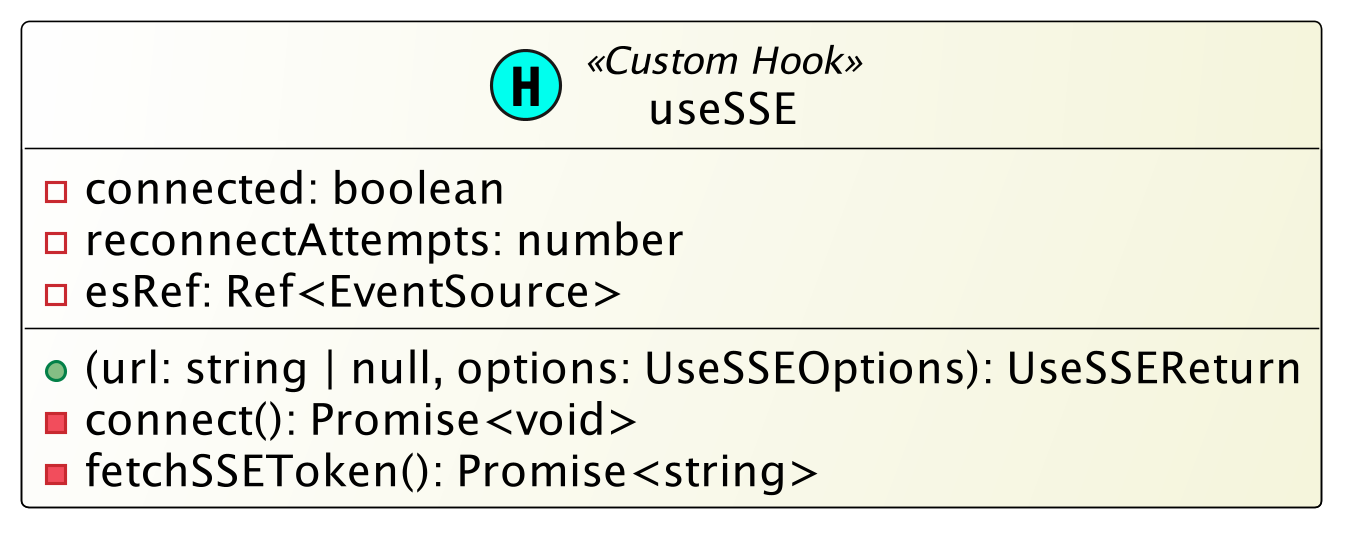
\includegraphics[width=0.62\textwidth]{componenti_specifiche_tecniche/assets/uml_frontend/06_useSSE.png}
    \caption{UML del modulo hook \texttt{useSSE}.}
\end{figure}

\paragraph{useHealthCheck / useProductSearch}
\vspace{\baselineskip}\noindent\textbf{Descrizione della classe:} moduli logici di corredo per separare lo stato del componente da computazioni esterne (la prima estendendo l'app sull'integrità del LLM, la seconda agendo da motore di query sul DB testuale/vettoriale riducendone il bounce).

\textbf{Descrizione degli attributi (Stati reattivi interni):}
\begin{itemize}
    \item \texttt{status}: enum \textit{loading $\vert$ ok $\vert$ error}.
    \item \texttt{searchTerm, results, isSearching}: payload di paginazione sui codici articolo.
\end{itemize}

\vspace{\baselineskip}\noindent\textbf{Descrizione dei metodi:}
\begin{itemize}
    \item \texttt{check(hook call)}: accetta cadenze (\texttt{intervalMs}).
    \item \texttt{doSearch(term)}: incapsula un debounce locale al client prima di trasmettere tramite \texttt{productService}.
\end{itemize}

\begin{figure}[H]
    \centering
    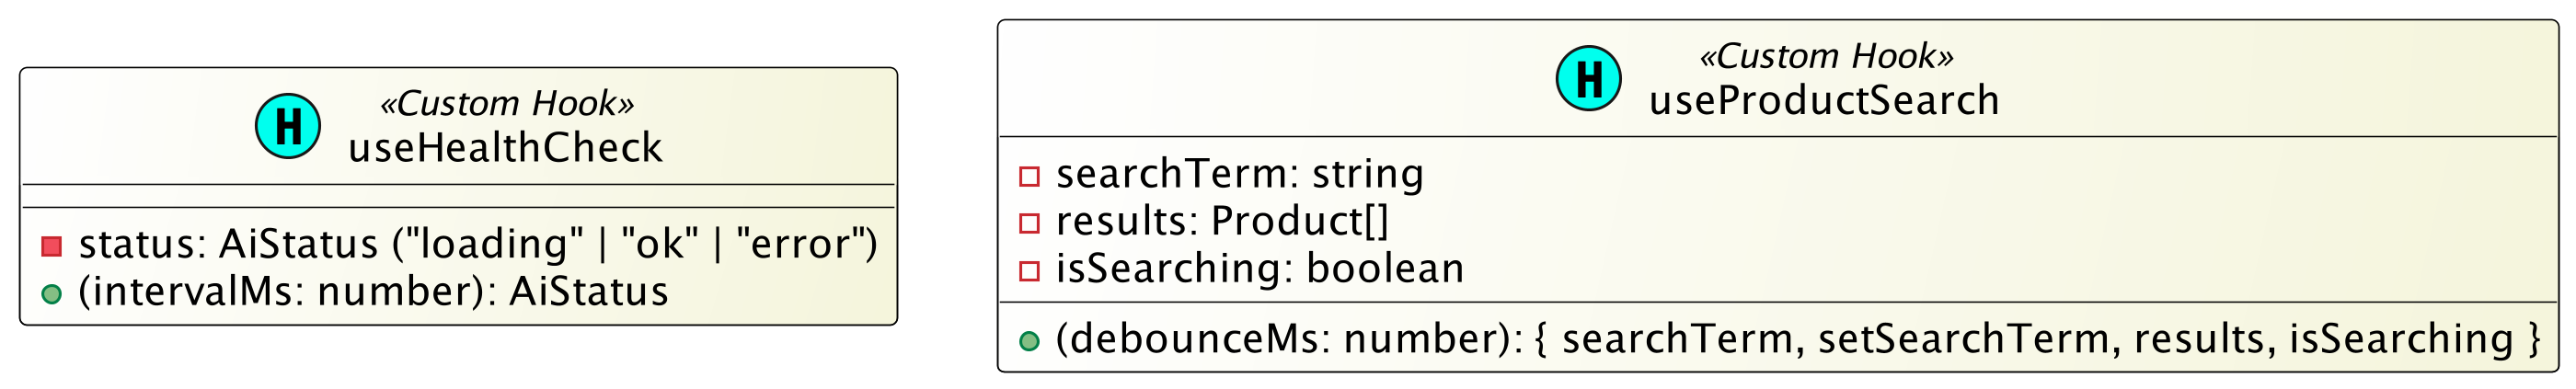
\includegraphics[width=0.62\textwidth]{componenti_specifiche_tecniche/assets/uml_frontend/12_otherHooks.png}
    \caption{UML dei restanti custom hook del frontend.}
\end{figure}

